\section{Experiments}
\subsection{Experimental setup}
\label{sec:setup}
\paragraph{Data.} We use the first public release of GUI-Odyssey~\citep{odysseyv1}, which contains 7,735 cross-app trajectories; the later ICCV version describes an expanded release~\citep{odysseypub}. We run EasyOCR on the screenshots of four sampled batches and mine cases as described in Section~\ref{sec:labels} (Table~\ref{tab:data}). The first batch samples trajectories that contain a candidate entry, the second and third target later steps, and the fourth takes trajectories of at least 16 steps with a candidate at $t\geq12$ while excluding all earlier batches. The first three batches form a development pool of 188 cases from 182 trajectories. We split it into five folds of 36--40 cases, keeping all cases of a trajectory in the same fold, train on four folds and predict the fifth; every development number below pools the five out-of-fold predictions. The fourth batch is a held-out set of 93 cases from 90 trajectories that share no episode with the development pool. For it, each selector is trained once on all 188 development cases and evaluated once. Most held-out cases occur at moderately late steps: 72 at $t=12$--15, 19 at $t=16$--19 and two at $t\geq20$.

\begin{table}[!htb]\centering
\caption{Sampling and case retention. Used trajectories are distinct episodes that contribute at least one retained case. The first three batches form the development pool.}
\label{tab:data}\small
\begin{tabular}{lrrrr}\toprule
Batch & Sampled trajectories & Candidate entries & Cases & Used trajectories\\\midrule
First & 300 & 431 & 85 & 81\\
Long & 300 & 355 & 53 & 53\\
Later-mined & 200 & 252 & 50 & 48\\\midrule
Development total & 800 & 1,038 & 188 & 182\\
Held-out batch & 400 & 438 & 93 & 90\\\bottomrule
\end{tabular}\end{table}

\paragraph{Baselines.} We compare the trained selectors with three prompted ones. The \emph{untrained per-screen} model uses the scorer's base model and prompt without the adapter, which isolates the effect of training. The \emph{full-history prompt} gives Qwen2.5-14B-Instruct the numbered history and asks for the source screen. The \emph{screen index}, inspired by ReadAgent~\citep{readagent}, has Qwen2.5-7B-Instruct write a one-line note of at most 20 words for every screen, naming the kind of screen and the kinds of values it shows but not the values themselves; the 14B model then picks a screen from these notes and reads its full OCR.

\paragraph{Metrics.} \emph{Localization} is the fraction of cases with $\hat i\in V_t$, so any screen that shows the answer counts as correct. \emph{Typed-text accuracy} is the fraction of cases in which the normalized generation contains the normalized reference text; periods are also removed for this check. A reader can pick the wrong field from a valid screen or recover the text from elsewhere in the history, so the two metrics capture different errors. All comparisons are paired on the same cases. We use two-sided McNemar tests with continuity correction and report nominal $p$-values from a single run per condition.

\subsection{Main results}
\label{sec:main}
Table~\ref{tab:main} reports localization and typed-text accuracy on the development pool and on the held-out set.

\begin{table}[t]\centering
\caption{Source-screen localization and typed-text accuracy (\%). The two 7B per-screen rows share the inference prompt and the reader. A dash marks a result that was not measured.}
\label{tab:main}\small
\begin{tabular}{lrrrr}\toprule
& \multicolumn{2}{c}{Development ($n=188$)}&\multicolumn{2}{c}{Held out ($n=93$)}\\
\cmidrule(lr){2-3}\cmidrule(lr){4-5}
Selector & Localization & Typed text & Localization & Typed text\\\midrule
Prompted screen index (14B) &41.0 &23.9 &37.6 &18.3\\
Prompted full history (14B) &54.8 &31.4 &59.1 &23.7\\
Untrained per-screen (7B) &50.0 &35.1 &41.9 & --\\\midrule
Trained full history (7B) &65.4 &42.6 &76.3 &\textbf{51.6}\\
Trained per-screen (7B) &\textbf{72.3} &\textbf{44.7} &\textbf{79.6} &49.5\\\bottomrule
\end{tabular}\end{table}

\paragraph{Derived labels make the per-screen model a much better selector.} With the base model, prompt and reader held fixed, training raises the scorer's development localization from 50.0\% to 72.3\%: 52 cases change from wrong to right and 10 from right to wrong ($p<0.001$). The same reader then types the correct text in 84 instead of 66 cases (23 gains and five losses, $p=0.0013$). On the held-out set, localization rises from 41.9\% to 79.6\%, so the gain carries over to unseen trajectories from the same corpus.

\paragraph{Both trained selectors outperform prompting.} The trained full-history selector localizes 123 of 188 development sources, compared with 103 for the 14B full-history prompt ($p=0.019$), although it uses a smaller model. On the held-out set, the scorer, the trained full-history selector and the full-history prompt localize 74, 71 and 55 of 93 sources, and the scorer's margin over the prompt is significant ($p=0.003$). The typed-text gaps to this baseline are larger but partly reflect the reading protocol, because the baseline's reader saw unmarked history in the first batch and only the selected screen elsewhere. A cleaner reading comparison keeps the trained scorer fixed and adds history to the reader, which raises held-out typed-text accuracy from 37.6\% to 49.5\% ($p=0.016$).

\paragraph{The two trained selectors are statistically close.} With a shared reader, the scorer finds 13 more development sources than the full-history selector ($p=0.086$) and types four more correct entries ($p=0.45$); on the held-out set the difference is three localizations ($p=0.63$). Both architectures benefit from the same labels, and the remaining difference between them is not statistically reliable.

\paragraph{Later steps are harder, and training narrows the drop.} At early steps ($t\leq15$, 75 cases), the full-history prompt, the trained full-history selector and the trained scorer localize 68.0\%, 76.0\% and 80.0\% of sources. At $t\geq16$ (113 cases), they localize 46.0\%, 58.4\% and 67.3\%. The step index counts the screens before the entry rather than the distance to the evidence, which we analyze in Section~\ref{sec:distance}.

\subsection{Finding the screen is not the same as reading it}
\label{sec:reading}
On the development pool, 74 of the scorer's 136 correct selections also yield the correct text, while in the other 62 the reader misses the value on a valid screen. Conversely, the reader recovers the text in 10 of the 52 cases with an invalid selection, because the unmarked history remains in its context. The held-out set shows the same pattern, with 43 of 74 correct selections yielding the right text and three recoveries after an invalid selection. The reader controls in Table~\ref{tab:controls} (right) show that reading is now the bottleneck: marking a screen known to be valid adds only one correct entry over the scorer's own choice (85 versus 84), whereas marking the most recent or a random earlier screen lowers accuracy to 38.8\% and 36.7\%. The reader must find the task-relevant field among many strings on a screen and copy it exactly. In Figure~\ref{fig:case}, both selectors chose valid screens, yet both readers missed the title.

\subsection{How far back does the model look?}
\label{sec:distance}
The answer recurs on several screens in 111 of the 188 development cases, so look-back distance has two natural definitions: the distance to the earliest match, $g_{\rm first}=t-\min V_t$, and the shortest sufficient look-back, $g_{\rm recent}=t-\max V_t$. Their medians are seven and four screens, and in Figure~\ref{fig:case} they are seven and five. Figure~\ref{fig:distance} partitions the same predictions under both definitions.

\begin{figure}[t]\centering
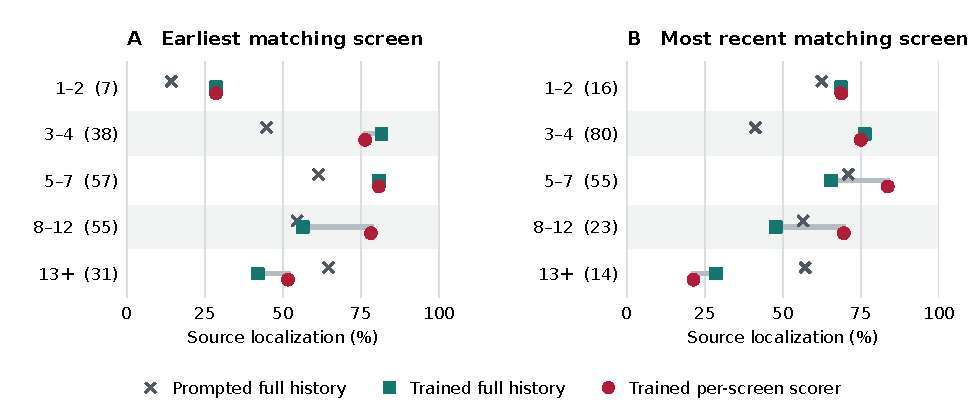
\includegraphics[width=\linewidth]{figures/distance.pdf}
\caption{Source localization by distance to the first (A) or the most recent (B) matching screen. Rows give distance ranges with case counts in parentheses. Both panels partition the same 188 development predictions.}
\label{fig:distance}\end{figure}

Grouped by $g_{\rm first}$, the scorer's advantage concentrates at 8--12 screens, where it finds 43 of 55 sources against 31 for the trained full-history selector (78.2\% versus 56.4\%; 13 improvements and one regression, $p=0.003$). Grouped by $g_{\rm recent}$, the same band holds only 23 cases and the difference (69.6\% versus 47.8\%) is not significant ($p=0.131$), because many cases with old earliest evidence also contain a recent copy (17 of the 31 cases with $g_{\rm first}\geq13$). On the 14 cases whose most recent evidence is at least 13 screens old, the full-history prompt finds eight sources, the trained full-history selector four and the scorer three. These groups are too small to support a precise cutoff for choosing between selectors, but they show that conclusions about distance depend on which occurrence is measured.

\subsection{Ablations and evaluation filters}
\label{sec:filters}
\begin{table}[t]\centering
\caption{Controlled variations on the 188 development cases. The left half changes the per-screen selector; the right half changes which screen the same reader sees marked in the history.}
\label{tab:controls}\small
\begin{tabular}{lr@{\hspace{1.4em}}lr}\toprule
Selector variation & Loc. (\%) & Reader highlight & Text (\%)\\\midrule
7B, distance, weight 3 &72.3 & Scorer's top screen &44.7\\
Omit distance header &70.7 & Scorer's top two screens &45.2\\
Positive weight 1 &72.3 & Known valid screen &45.2\\
Smaller 3B model &68.1 & Most recent screen &38.8\\
 & & Random earlier screen &36.7\\\bottomrule
\end{tabular}\end{table}

\paragraph{Selector ablations.} The left half of Table~\ref{tab:controls} varies the scorer. Removing the explicit distance from the prompt changes localization by 1.6 points ($p=0.61$), and equal class weights leave it unchanged, so the result is not sensitive to these choices. A 3B scorer finds fewer sources overall (68.1\%) but more at $t\geq20$, where it reaches 48.1\% (13 of 27) against 37.0\% for the 7B scorer.

\paragraph{Why a screen index falls short.} In the example of Figure~\ref{fig:case}, the notes for screens 4, 5 and 6 list only kinds of values (\emph{name, url, station, playlist, \ldots}) and never the title itself. On the first 85 cases, the prompted one-line-per-screen index localizes 49.4\% of sources, compared with 65.9\% for prompting with the full OCR. Training the line writer with preference optimization does not close this gap (45.9\%), even though its preference pairs reuse the evaluation set, and four writer variants range from 43.5\% to 49.4\%. A BM25 retriever queried with the task and the current screen finds 10.6\% of sources but 92.9\% when queried with the hidden answer, which shows that the difficulty lies in not knowing what to search for.

\paragraph{Two evaluation filters change conclusions.} First, 40 of the first 85 cases have several valid screens; crediting only the earliest one would understate the screen index by 15.3 points and the full-history prompt by 11.8. Second, cases whose answer is still on the current screen reward any method that reads recent screens. On the unfiltered 127-case long batch, a recent-screen gating rule beat the full-history prompt by 17.3 points, but after removing the 74 leaked cases it trailed by 22.7 points on the remaining 53, and we withdrew that earlier finding.
